%!TEX program = lualatex

\documentclass{tufte-handout}
\usepackage{hyperref}
\usepackage{amsmath}
\usepackage{titlesec}
\usepackage{framed}
\usepackage{todonotes}
\usepackage{arydshln}
\usepackage{fontawesome}
\usepackage{fontspec}
\usepackage{pdfpages}
\usepackage{csquotes}
\MakeOuterQuote{"}
\setmainfont{Palatino Linotype}

\titleformat
{\part} % command
[display] % shape
{\bfseries\Large\itshape} % format
{Story No. \ \thechapter} % label
{0.5ex} % sep
{
    \rule{\textwidth}{1pt}
    \vspace{1ex}
    \centering
} % before-code
[
\vspace{-0.5ex}%
\rule{\textwidth}{0.3pt}
] % after-code

% Set up the images/graphics package
\usepackage{graphicx}
\setkeys{Gin}{width=\linewidth,totalheight=\textheight,keepaspectratio}
\graphicspath{{syllabus-img/}}

\title{Teaching with Digital Media and Technology}
\author{Dr. Jeremy Price}
\date{Spring 2015}  % if the \date{} command is left out, the current date will be used

% The following package makes prettier tables.  We're all about the bling!
\usepackage{booktabs}

% The units package provides nice, non-stacked fractions and better spacing
% for units.
\usepackage{units}

% The fancyvrb package lets us customize the formatting of verbatim
% environments.  We use a slightly smaller font.
\usepackage{fancyvrb}
\fvset{fontsize=\normalsize}

% Small sections of multiple columns
\usepackage{multicol}

% Provides paragraphs of dummy text
\usepackage{lipsum}

\usepackage{microtype}

% These commands are used to pretty-print LaTeX commands
\newcommand{\doccmd}[1]{\texttt{\textbackslash#1}}% command name -- adds backslash automatically
\newcommand{\docopt}[1]{\ensuremath{\langle}\textrm{\textit{#1}}\ensuremath{\rangle}}% optional command argument
\newcommand{\docarg}[1]{\textrm{\textit{#1}}}% (required) command argument
\newenvironment{docspec}{\begin{quote}\noindent}{\end{quote}}% command specification environment
\newcommand{\docenv}[1]{\textsf{#1}}% environment name
\newcommand{\docpkg}[1]{\texttt{#1}}% package name
\newcommand{\doccls}[1]{\texttt{#1}}% document class name
\newcommand{\docclsopt}[1]{\texttt{#1}}% document class option name

\newcommand{\tabpq}{\faQuestionSign\medspace\textit{Priming Questions}}
\newcommand{\tabread}{\faBook\medspace\textit{Readings}}
\newcommand{\tabtools}{\faWrench\medspace\textit{Tools}}
\newcommand{\tabtweet}{\faLightbulb\medspace\textit{Reflection Task} & Surprise Tweet Due Friday \\}
\newcommand{\tabcheck}{\faLightbulb\medspace\textit{Reflection Task} & Metacognitive Check Due Friday (no Surprise Tweet) \\}
\newcommand{\tabperformance}{\faTasks\medspace\textit{Performances}}
\newenvironment{tabsched}
	{\small
	\begin{tabular}{p{1.5in}p{4.5in}}
	\toprule}
	{\bottomrule
	\end{tabular}
	\normalsize}

\newenvironment{specweek}
	{\begin{center}
		\fontseries{b} \faBullhorn \medspace Special Week: }
		{\medspace \faBullhorn \fontseries{m}
	\end{center}}

\newcommand{\weekone}{August 17-21}
\newcommand{\weektwo}{August 24-28}
\newcommand{\weekthree}{August 31-September 4}
\newcommand{\weekfour}{September 7-11}
\newcommand{\weekfive}{September 14-18}
\newcommand{\weeksix}{September 21-25}
\newcommand{\weekseven}{September 28-October 2}
\newcommand{\weekeight}{October 5-9}
\newcommand{\weeknine}{October 12-16}
\newcommand{\weekten}{October 19-23}
\newcommand{\weekeleven}{October 26-30}
\newcommand{\weektwelve}{November 2-6}
\newcommand{\weekthirteen}{November 9-13}
\newcommand{\weekfourteen}{November 16-20}
\newcommand{\weekfifteen}{November 30-December 4}
\newcommand{\laborday}{Labor Day on Monday, September 7 (no class)}
\newcommand{\roshhashanah}{Rosh Hashanah on Monday, September 14 (class via VoiceThread)}
\newcommand{\yomkippur}{Yom Kippur on Wednesday, September 23 (class via VoiceThread)}
\newcommand{\midsemester}{Mid-Semester Point}
\newcommand{\acmhe}{Dr. Price at ACMHE Conference on Friday, October 9 (class via VoiceThread)}
\newcommand{\thanksgiving}{Thanksgiving Recess, November 23-27 (no class)}
\newcommand{\finisemester}{Last Day of Class, Friday, December 4}

\begin{document}

\maketitle% this prints the handout title, author, and date

\marginnote{\textit{What is a syllabus?} The syllabus is your map for success in this course. It provides you with the course practices and expectations, a schedule for readings and assignments, and a breakdown of the points you can earn in the class. Put your syllabus in your binder and \emph{bring your syllabus with you to class everyday.}}

\begin{abstract}
Welcome to EDUC2201, Teaching with Digital Media and Technology. We will be exploring the different ways that technology can be used to support learning, understanding, and creativity in the classroom or in other types of learning environments. We will be paying special attention to the role that you play as facilitator and intentional designer of materials and of the environment to encourage learning, understanding, and creativity.\end{abstract}

%\addvspace{1.5in}
\bigskip

\begin{fullwidth}
\begin{center}

	
\includegraphics[width=0.20\linewidth]{twt-logo.png}

	\bigskip

	\Large
	\enquote{Teaching is two-parts planning, one-part reflection, and extra heavy on the experimentation.}~-~Rebecca Alber

	\bigskip

	\enquote{It seems to me that that, finally, is what good teaching is all about\ldots~~Somehow or another, skill and knowledge are integrated into some kind of a human connection.}~-~Mike Rose

	\normalsize
\end{center}
\end{fullwidth}

\vfill

\subsection{Get to Know Your Professor}

\noindent Dr. Jeremy Price

\noindent Office: Education 315 | 304.333.3686

\noindent \marginnote{\textit{Psst: Email is the best way to contact me.}}Email: \href{mailto:jeremy.price@fairmontstate.edu}{\nolinkurl{jeremy.price@fairmontstate.edu}}

\noindent Visit me during my student drop-in hours:
\marginnote{If you can't make my student drop-in hours, schedule an appointment with me at \url{https://jeremyprice.youcanbook.me/}}
\begin{table}[ht]
  \centering
  %\fontfamily{ppl}\selectfont
  \begin{tabular}{ccc}
    \toprule
    Mondays & Wednesdays & Fridays \\
    \midrule
    10:00am - 12:00pm & 10:00am - 12:00pm & 10:00am - 12:00pm \\
    \bottomrule
  \end{tabular}
\end{table}
\newpage

\part{The EDUC2201 Contract}
\begin{fullwidth}

\textit{\textbf{Your first job} is to work at developing an academic relationship with me as your professor} just as you should work to develop a relationship with all of your professors. This job for you extends to \emph{all} of your classes; you will find that putting the effort into building an academic relationship with your professors pays off. Putting effort into building an academic relationship with your professor will make your other two jobs flow much more smoothly. I am (and all of your professors are) here to help you succeed. In order to help me support you, you need to help me know what you need. If you have a question, if you don't understand something, if you are having trouble getting to class, if you need a different explanation of something, \emph{talk to me}. Sometimes this means coming to my Student Drop-In Hours or scheduling an appointment with me outside of class. I work very hard to get to know my students in class, but I get to know them even better (and I can provide more targeted support) when my students talk with me outside of class.

\textit{\textbf{Your second job} is to get to know and learn how to use all of the course materials.} I will provide you with information, models, and scaffolding in the syllabus and other companion documents. These companion documents include \texttt{Reference Sheets}, \texttt{Project Packages}, and \texttt{Model Assignments}. Success in this class involves organizing and understanding these sources of information; we will go over the syllabus in depth during the first class, and I am happy to meet with you to discuss the course and its requirements further.

\textit{\textbf{Your third job} is to consider the long-term returns you will gain from putting effort into the work of this course.} When you are in college, your primary work responsibilities are to your coursework. You are in the Teacher Education Program and the effort you put into your coursework will pay off in terms of becoming a better prepared and more successful teacher. It is hard to find a balance between these long-term payoffs and short term needs (such as paying for rent, clothing, or entertainment and fun activities). You may also be more responsible for your time and attention than you ever have been before, so it is easy to slip into a pattern of missing classes, sleeping in, or spending late nights at parties. I am more than happy to help you find the right balance and to connect you with people and resources than can provide further support.

\textit{\textbf{My jobs as your professor}} include designing an engaging, relevant, productive course, facilitating class activities that I believe will be effective in the learning process, assessing your work in a fair, timely manner, and creating a safe, supportive space in which everyone can be who she or he is and freely contribute to the class. I am here to support you as you succeed in this course and in the Teacher Education Program, but I can only do so with your help.

\end{fullwidth}
\newpage

\part{Becoming a Teaching Superhero}

\begin{marginfigure}%
	\begin{center}
		
\includegraphics[width=0.75\linewidth]{teach-superpower.png}
		\label{fig:teach-superpower}
	\end{center}
\end{marginfigure}


\newthought{I want to help you to become teaching superheroes with technology.} The children and young adults with whom you will be working deserve nothing less. In order to help you get there, we will be supporting you along the way to develop the practices and routines, digital tools, and knowledge for teaching necessary to be teaching superheroes with technology and getting accepted into the Teacher Education Program in the School of Education, Health and Human Performance at Fairmont State University. We will work hard together to accomplish that goal.

\subsection{Course Throughlines}
\marginnote{Using vocabulary of the profession is important and will help you communicate with your professors and colleagues in a precise and professional manner. We will therefore be using the ideas and language of the Teaching for Understanding (TfU) framework. According to TfU, \textit{throughlines} \enquote{describe the most important understandings that students should develop during an entire course.} Throughlines are the big ideas that we will be exploring and developing understandings around over the semester.}

\begin{center}
	\large\textit{In this course, we will explore the questions\ldots}
\end{center}
\begin{framed}
	\small
	\begin{itemize}
		\item How do I see my role as a teacher with technology?
		\item How do I relate teaching, technology, and me?
		\item What practices and routines, digital tools and knowledge for teaching can I develop to support my role as a teacher with technology?
	\end{itemize}
\end{framed}
\begin{center}
	\large$\downarrow$\hspace{0.5em}\textit{By engaging in these experiences\ldots}\hspace{0.5em}$\downarrow$
\end{center}
\begin{framed}
	\begin{center}
		
\includegraphics[width=0.45\linewidth]{experiences.png}
	\end{center}
\end{framed}
\begin{center}
	\large$\downarrow$\hspace{0.5em}\textit{To help you become\ldots}\hspace{0.5em}$\downarrow$
\end{center}

\begin{framed}
	\begin{center}
		\small\noindent\textbf{A thoughtful educator who uses technology to support learning by facilitating the growth of understanding and creativity in each learner.}
	\end{center}
\end{framed}

\normalsize

\newpage

\part{Course Practices and Routines}

\begin{marginfigure}%
	\begin{center}
		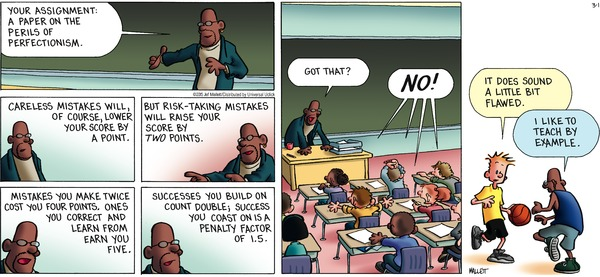
\includegraphics[width=1\linewidth]{frazz-mistakes.png}
	\end{center}
\end{marginfigure}

\section{A Commitment to Universal Learning}
\newthought{I am committed to the principle of universal learning.} This means that our classroom, our virtual spaces, our practices, and our interactions be as inclusive as possible. Mutual respect, civility, and the ability to listen and observe others carefully are crucial to universal learning.

Any student with particular needs should contact the coordinator of Disability Services at the start of the semester. Services are available to any student, full or part-time, who has a need because of a [documented] disability.\marginnote{The coordinator of Disability Services can be reached at 304.367.4686 or 800.641.5678 Ext. 8.} It is the student's responsibility to register for services with the coordinator of students with disabilities and to provide any necessary documentation to verify a disability or the need for accommodations.  You and I can work out the details of any accommodations for this course.

\section{Improve Your Chances for Success by Coming to Class Every Day}
\newthought{Being present is important to success in this class.}\footnote{Research has found that just showing up to class is a better way to tell if you will do well in your college classes than anything else, including how you might have done in high school (Crede, Roch, and Kieszczynka, 2010).} This class is very collaborative and you will often be working in teams: your teammates depend on you. Attendance will be taken at every class, both as a way to help me learn your names and as a way to help you stay on track with attendance.

I also understand that life happens and sometimes you might need to miss class. \footnote{\textit{Some acceptable reasons to miss class} include family emergencies, car troubles break down, icy or snowy roads, or illness. \textit{Some not acceptable reasons to miss class} include oversleeping, conflict with outside jobs, or the \enquote{I don't feel like going to class} excuse.} Keep an open line of communications with me about your absences from this class. \textbf{If you need to miss class, please notify me directly by email}. Although I would prefer to be notified ahead of time of your absence, if you have an excuse for your absence you have 24 hours after class to notify me. I will notice patterns of absences\textemdash{}unexcused \emph{and} excused\textemdash{}and I will call you on it because I want to do everything I can to help you succeed.

\subsection{Building Trust: \enquote{Ooops!} Days}
You might forget me to send me an email, so \textbf{each teacher candidate in EDUC2201 receives two "Ooops!" days.} Each unexcused absence beyond your two "Ooops!" days will result in 50 points taken off your final grade for the course.\marginnote{If you earned an B in the course but had two unexcused absences beyond your two "Ooops!" days, you will receive a C for your final grade.} \emph{If you need to be excused from class for an extended period of time} for a particular reason, you must speak to me directly outside of class\textemdash{}such as during my drop-in hours, or if you can't come at those times, schedule an appointment with me\textemdash{}so that we can work out a way for you to participate in the structure and activities of the course. I will be posting your attendance status on TaskStream each month.

\newthought{The most important thing is to keep an open line of communications open with me:} I am here to help you succeed. I recognize that students are required to miss class for many different reasons. The important thing to remember is to keep an open line of communications with me so your grade is not adversely affected.

\section{Be Better Prepared for Class with Active Reading}
We will be reading a series of articles from educational journals and blogs each week. You are expected to complete readings prior to the start of class; if you do, you will be better prepared and be able to participate more fully in the discussions. We will be discussing these readings in class, drawing upon their ideas and concepts, and you will be asked to support your statements with evidence from the readings. I will also help you to make sense of these readings by helping you find the important and salient concepts. I recommend using the \textsf{SQ3R Method} for reading for this course (and all courses), which is illustrated and described in the \textsf{Course Tools and Practices} companion document.

\section{Get in the Right Groove for Class}
Every class will begin with a \textsf{cognitive warm-up}, a short activity designed to you make the transition into class and to help everyone get on the same page for a successful class. Many of the activities are designed to \textit{activate your prior knowledge} and \textit{prime you}\footnote{\textit{Prior knowledge} is the knowledge that you bring with you to your school work. \textit{Priming} is getting you in the right mindset to engage in the work at hand.} for the work to follow. Most students have said that this helps them prepare and participate in each class. So, \textit{arriving on time is important} and is a sign of respect to your classmates and to your professor. If you arrive during the cognitive warm-up, please wait outside in the hall until the activity is over. Use this time to take a deep breath and mentally prepare for class until the activity is over, when you are welcome to come in and find a seat.

\section{Participate Effectively to Get More Out of Class Time}
\newthought{We learn best} when we converse with others about ideas and concepts, and participation is an important practice for success in university academic life in general. Ongoing participation is an important and required practice in this course. I understand that this may be out of some students' comfort level, but as you will be educators in the near future, I want to help you develop the skills and confidence to lead a discussion and take intellectual risks\footnote{Another way of thinking about \textit{intellectual risks} is contributing without the fear of being 100\% right. As Ms. Frizzle of the \textit{Magic School Bus} once said, "Take chances, make mistakes, get messy!"}. Teaching is also a highly collaborative career, meaning that you will be working closely with other teachers, school and district administrators, your students and parents just to do your job. The EDUC2201 classroom is a safe environment in which to practice participation skills.

\emph{Quality participation does not mean that you talk the most, or even responding to my questions all the time.}\marginnote{Technology is a wonderful tool, but it is also a way to avoid being present. There is no texting allowed in class, and I will notice when you use the laptops and tablets for reasons other than the task at hand, such as checking Facebook, playing games, or shopping.} Some of the behaviors that show me that you are developing strong participatory and collaborative practices include:
\begin{itemize}
	\itemsep-0.5em
	\item \textbf{Asking questions}
	\item Responding to a \textbf{fellow student}
	\item \textbf{Providing assistance} or helping another student
	\item Making comments drawn from the \textbf{course readings}
	\item Agreeing or disagreeing with something in the text or said in class by the instructor or another student in a way that \textbf{takes the conversation to a new level}
\end{itemize}
It is good to "answer questions" (and sometimes I will ask the class a question to better understand the current level of understanding) and it is often good to draw on your personal experience. But there's more to it than that; participation also involves bringing in what you have learned from the readings and applying what you learn from the in-class discussions to your Learning Performances.

\section{Take Knowledge from Class to Projects by Taking Notes}
We will be discussing a number of important ideas in class that you will need to use in your assignments and projects. I will be asking you to write how you used the ideas we discussed in class to complete your projects, the more specific the better. There are a number of ways to take notes but the most important thing is that you find the method of note-taking that works for you. Remember that \emph{effective note-taking is more than writing down bullet points from PowerPoint slides}.

\newthought{To help you develop the practice of note-taking,} I will be asking you to cite specific information from class and from the readings in your \textsf{Reflection Write-Ups} for your \textsf{Performances of Understandings}. Taking notes will help you to refer back to our discussions and use them in your \textsf{Reflection Write-Ups}. An important part of becoming a successful learner is moving ideas from one context to another, and I hope that this process will help you build some of the same practices with your own students in the future.

\section{Stay Current by Keeping In Touch Outside of Class}

\newthought{Communications between me and you outside of class will occur over \underline{email}.} \marginnote{If you wish to be notified by text every time I send an email to the class, please send a text to 81010. If you are in the 9:00am class, send the message \texttt{@edu2201-9}. If you are in the 12:00pm class, send the message \texttt{@edu2201-12}.}Please do not send me a message through Blackboard. Please make sure to check your Fairmont State email on a regular basis (at least 4-5 times per week). If you do not have a smart phone, a computer or internet access at home or in your dorm room, make it a regular practice to go to the library and check your email there.

\begin{figure}%
  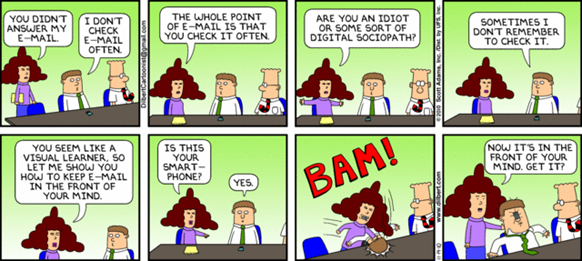
\includegraphics[width=\linewidth]{dilbert-email.png}
  \caption{Don't be like Ted: check your email and check it often.}
  \label{fig:dilbert-email}
\end{figure}

\section{Learn More by Submitting Assignments and Making Good Use of Feedback}
\newthought{It is important to submit assignments on time} as a professional courtesy to yourself, your professor, and your classmates. All assignments are due in TaskStream before \textit{Pumpkin Hour}\footnote{\textit{Pumpkin Hour} is 11:59pm on the day the assignment is due.}. It is best not to wait until the Very Last Minute to submit assignments on \texttt{TaskStream}, as the submission process requires several steps.

I completely understand that life happens and emergencies, illnesses, and other situations come up when you least want them to.\marginnote{The \textit{Things Happen Buffer} gives you a little wriggle-room when it comes to handling the things that come up in life. Make sure to send me an email within \emph{24 hours} after the due date if something comes up. The sooner you contact me the better.} If you are involved in an emergency, illness, or situation, please inform me via email as soon as possible, preferably before the due date, and we can discuss an extension. I also understand that things may happen on the date an assignment is due, so every student in EDUC2201 has a \textit{Things Happen Buffer}.

%\marginnote{Yes, I will give extensions for good reasons. Try me.}

\subsection{Keeping the Learning Going by Reviewing Your Feedback}
I spend a great deal of time and effort reviewing your work and providing feedback that I think will be helpful for you. \marginnote{\textit{There is no shame in resubmissions.} Making adjustments to your work is part of the learning process. I also agree with educator Richard Curwin who says that education should really be about giving students second, third, fourth chances\ldots}There is also a possibility that you did not fulfill the requirements of the task; in this case, I will ask you to revise and resubmit your work through TaskStream before I assign you points. If you don't check TaskStream and look at your feedback, you won't know this.

\newthought{You can learn a great deal from feedback} so it is important to take the time and effort to read it closely. I \emph{critique} your work, meaning that I provide information about what you did well and information for helping you to do better work in the future. Use this feedback to improve your work in other assignments because the learning performances in this class are related to each other. \marginnote{You have one week from the time I provide you with feedback to resubmit your work for review.}\textbf{\emph{You always have the option of resubmitting your work if you feel that you have learned from my feedback and want to show me what you have learned.}}

\newpage

\part{Performances of Understanding}

\begin{marginfigure}%
	\begin{center}
		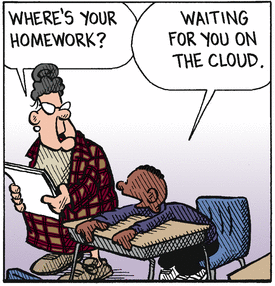
\includegraphics[width=1\linewidth]{frazz-homework.png}
	\end{center}
\end{marginfigure}

\newthought{Performances of Understanding are a way for you to demonstrate what you understand while also building your understanding.} These performances can be ongoing short check-ins or projects that can take anywhere from 2 to 5 weeks to complete.

\section{Become a Scholar by Building Your Metacognitive Skills}
\newthought{Metacognition means "thinking about thinking."} Being aware of your own thinking will help you learn more and help you succeed throughout your college career. It is also something that I hope you will help your own students develop when you are a teacher. Metacognition happens in part through (1)~setting goals, (2)~being intentional about your effort, and (3)~reflecting on your learning.

\subsection{Learning Tweets}
You will be writing a "Learning Tweet" each week. You won't be using Twitter to write your tweets (you will be writing it directly to me using \texttt{TaskStream}), \marginnote{Your Learning Tweet should be a little longer than the typical tweet on Twitter: no less than three sentences.}but just like Twitter your Learning Tweet will be on the short side. You will be asked to post a Learning Tweet during some weeks directly on the readings, some weeks on class discussions, and some weeks on anything from class that surprised you. \emph{Make sure that your Learning Tweets have something to do with \textbf{this} class}.

The task of each Learning Tweet will be provided in TaskStream. The structure of the general Learning Tweet that focuses on something from the class that surprised you will follow the \texttt{Moment of Surprise}, \texttt{Why It Was Surprising}, and \texttt{What This Tells Me} format:

\begin{itemize}
	\itemsep-0.5em
	\item \texttt{Moment of Surprise:} a short summary of the reading, discussion, or activity you are writing about;
	\item \texttt{Why It Was Surprising:} a short description of what about the reading, discussion, or activity caught your attention, surprised or intrigued you;
	\item \texttt{What This Tells Me:} your "take away" from this surprise, what you learned, how your perspective has changed.
\end{itemize}

The Learning Tweets allow you to make sense of your experiences and gives me a sense of what you are taking away from the class. I often readjust my teaching based on what students tell me through the Surprise Tweets. Keeping track of these "surprises" is a form of ongoing reflection and is an essential component of learning and teaching. We will be reading a short article on surprises in learning during the first week.

\medskip\noindent\textit{$\mapsto$~Each Surprise Tweet is worth 10 points, for a total of 120 points.}

\subsection{Metacognitive Self-Checks}

You will complete a \texttt{Metacognitive Self-Check} at three points in the semester to allow you to reflect on your learning and participation practices for the class. You will choose three metacognitive practices that you wish to improve on over the course of the semester. You will then complete a rubric on these three practices,\marginnote{The Beginning-Developing-Succeeding rubric scale is based on educational psychologist Carol Dweck's idea of a \textit{growth mindset}. Adopting a growth mindset will help you recognize that you continuously learn.} rating yourself on a scale of Beginning-Developing-Succeeding. These Self-Checks will also allow me to see how you see yourself as a learner and a member of the class and allow me to provide you with added feedback, support and resources to help you succeed as a learner in the course and in college in general. Many students have found this to be a useful way to help them focus on improved participation in the class. You will not have to complete a Learning Tweet when a Metacognitive Self-Check is due.

\medskip\noindent\textit{$\mapsto$~Each Self-Check is worth \textbf{20 points}, for a total of \textbf{60 points}.}

\subsection{Reflection Write-Ups}

Reflecting on your work and your practice is an important part of being a teacher. I will help you develop these skills through structured reflections on your experiences throughout the semester. Each reflection will follow a slightly different structure, so make sure that you look closely at what is required of teh reflection. The basic parts of a reflection involve \texttt{framing} and \texttt{reframing}. \marginnote{\textit{Framing} refers to describing in detail the way that your project was completed. \textit{Reframing} refers to describing in detail how you\textemdash{}or a make-believe educator\textemdash{}might use your project in the future.}This method of reflection will allow you to look back on what you've done as well as project into the future as to how you might use what you have learned in your own teaching practices.

\medskip\noindent\textit{$\mapsto$~Each Reflection is worth \textbf{10\% of Culminating Performance points}. The Reflection Write-Up is a required part of the project process and your submission will be returned to you if you do not also submit a Reflection Write-Up.}

\subsection{Passport Activities}
Fairmont State University is looking to improve the learning experience of all students and help students build a successful academic career from admissions to graduation. Part of building this success is to become involved in campus life. As such, as a student in this course, you will \marginnote{Certain individuals who are already participating in the life of the University may qualify for an exemption.}required to participate in the Fairmont State Passport Program. You are required to create a plan of action for attending Passport Activities over the course of the semester and attend them. Of these activities, you will attend one of two "core" activities \marginnote{The two core activities are Dr. Sidwell's \textit{Personal Health \& Safety Plan} or Dr. Rohrbaugh's \textit{The Human Brain: Studying for University Classes}.}and write a reflection on your experience. You will also attend \textit{\textbf{four additional Passport Activities}}. The Passport Activities options will be provided for you early in the semester. If you have a Passport Activity you would like to organize, please let me know.

\medskip\noindent\textit{$\mapsto$~Attendance at a Passport Core Activity and the written reflection is worth \textbf{60 points}. Attendance and short reflections at four additional Passport Elective Activities are worth 10 points each for a total of \textbf{40 points}.}

\section{Intermediate and Culminating Performances of Understanding}

The \textit{Performances of Understanding}\footnote{Performances of Understanding are a concept from the Teaching for Understanding framework. You will be learning about this framework in depth during Unit 4 (The Quest to Build a WebQuest).} are what you produce in each of the 5 units of the course. Each of these Performances are designed to not only help me see what you understand, but also to help you deepen your knowledge and develop your skills around the use of technology in teaching and learning. You will receive a \textsf{Project Package} at the beginning of each unit which will include more specifics about what I expect from you, including a copy of the rubric that I will be using to evaluate your work. In addition to the Culminating Performances themselves, you will engage in Intermediate Performances to help you get ready for the Culminating Performances.

\subsection{Unit 0: Getting Started and Situated}

The first week of class will be dedicated to helping everyone get into the flow of the course. We will be establishing expectations and practices for the semester. You will be completing an open-syllabus "quiz." This will allow you to get familiar with the syllabus, the expectations of the class and \texttt{TaskStream}.

\medskip\noindent\textit{$\mapsto$~Your Syllabus Quiz is worth \textbf{10 points}.}


\subsection{Unit 1: Communicating the Role of Technology in Education}

This first unit will introduce you to the idea of technology in education and challenge you to consider why using technology to support learning is important. This unit is also structured to help you succeed on the Praxis Core Academic Skills for Educators Exam. The essay you will write is similar to the argumentative essay you will write for the Core Exam. I will be helping you through the writing process that you can then bring into your own classrooms to support your own students when you are a teacher. In addition to writing the essay, I will be requiring you to accomplish two other steps: \textit{take a draft of your paper to the Writing Center} and \textit{meet with me to discuss the feedback on your paper}. The Writing Center is an excellent free on-campus resource for you. In our meeting, I will help you make good use of the feedback on your essay and it will help us get to know each other better.

\medskip\noindent\textit{$\mapsto$~Your visit to the Writing Center is worth \textbf{40 points}. Your Argumentation Essay Culminating Performance is worth \textbf{90 points}.}

\subsection{Unit 2: Creating an Online Book for All Learners}

As a way to engage in digital authoring and inclusive digital practices, you will write an online book for high school or college students about a time when you felt like you persisted, belonged, or saw things in a new way in order to succeed in a learning (although not necessarily classroom) environment. Helping students persist, develop a sense of belonging, and seeing ideas or problems in new ways has been shown to support academic achievement; this unit will help you explore your own experiences as well as help to prepare you to impress the value of the same practices on your future students.

\medskip\noindent\textit{$\mapsto$~Your Outline is worth \textbf{20 points} and your Storyboard is worth \textbf{40 points}. The Online UDL Book is worth \textbf{150 points}.}

\subsection{Unit 3: Exploring the Many Sides of Diversity}

Fully understanding\textemdash{}and supporting\textemdash{}diversity in the classroom will help you become a more successful teacher. This WebQuest will lead you through a number of activities to help you recognize, understand, and advocate for classroom diversity. You will be working as a team to create a public exhibit illustrating diversity through music. You will also become familiar with the structure of WebQuests.

\medskip\noindent\textit{$\mapsto$~Your Diversity Poster Culminating Performance is worth \textbf{90 points}.}

\subsection{Unit 4: The Quest to Build a WebQuest}

As a way to engage in constructing digital learning environments and "get your feet wet" in using the Teaching for Understanding framework, you will construct a well-structured WebQuest for elementary, middle, or high school pupils on a particular topic of your choosing. As part of the process, you will create a "map" with Prezi using the Teaching for Understanding framework. You will also use additional media from other digital tools covered over the course of the semester in your WebQuest.

\medskip\noindent\textit{$\mapsto$~Your TfU Map Intermediate Performance is worth \textbf{100 points}. Your WebQuest Culminating Performance is worth \textbf{180 points}.}

\section{Course Point Breakdown}

\marginnote{900-1000 points is an A, 800-899 points is a B, 700-799 points is a C, 650-699 is a D, 649 or less is an F.}Keep in mind that \emph{\textbf{you earn your grade}}. I do not "give" you a grade. As a teacher, I place a great deal of emphasis on becoming aware of learning processes and progress. \emph{This is a practice that is important to bring to your own students,} so I want to give you a head start.

\bigskip

% The following scores in the table are correct and add up to 1000 (7/28/2015)

\begin{tabular}{clr}
	\toprule
	Unit & Performance & Points \\
	\midrule\midrule
	0 & Syllabus "Quiz" & 10 \\
	\midrule
	1 & Writing Center Feedback Intermediate Performance & 40 \\
	& Argument Paper Culminating Performance & 90 \\
	\midrule
	2 & Outline for UDL Book Intermediate Performance & 20 \\
	& Storyboard for UDL Book Intermediate Performance & 40 \\
	& UDL Book Culminating Performance & 150 \\
	\midrule
	3 & Diversity Poster Culminating Performance & 90 \\
	\midrule
	4 & Prezi Teaching for Understanding Map Intermediate Performance  & 100 \\
	& WebQuest Culminating Performance & 180 \\
	\midrule
	MC & Preparatory \& Reflection Tweets (Total) & 120 \\
	MC & Metacognitive Checks (Total) & 60 \\
	MC & Passport Core Activity & 60 \\
	MC & Passport Elective Activities (Total) & 40 \\
	\midrule\midrule
	\multicolumn{2}{l}{\textbf{Total}} & \textbf{1000} \\
	\bottomrule
\end{tabular}

\newpage

\part{\faCalendar\medspace Course Schedule \medspace\faCalendar}

\begin{marginfigure}
	\begin{center}
		
\includegraphics[width=0.4\linewidth]{frazz-time.png}
	\end{center}
\end{marginfigure}

\medskip

\section{Intermediate and Culminating Performances of Understanding Due Dates}
\begin{tabular}{clr}
	\toprule
	Unit & Performance & Due Date \\
	\midrule\midrule
	0 & Syllabus "Quiz" & January 26 \\
	\midrule
	1 & Writing Center Feedback Intermediate Performance & February 13 \\
	& Argument Paper Culminating Performance & February 20 \\
	& Meeting with Professor & March 15 \\
	\midrule
	2 & Outline for UDL Book Intermediate Performance & February 23 \\
	& Storyboard for UDL Book Intermediate Performance & February 27 \\
	& UDL Book Culminating Performance & March 13 \\
	\midrule
	3 & Diversity Poster Culminating Performance & March 27 \\
	\midrule
	4 & Prezi Teaching for Understanding Map Intermediate Performance  & April 13 \\
	& WebQuest Culminating Performance & May 1 \\
	\bottomrule
\end{tabular}

\section{Unit 0: Getting Situated and Started}

\subsection{Week of \weekone}

\begin{tabsched}
	\tabpq & What are some of the rules of the "program" for "doing school"? \\
	& Should an effort be made to "deprogram" students from "doing school"? \\
	& What does the author mean by "surprise," and why is surprise important for learning? \\
	\midrule
	\tabread & How Deprogramming Kids From How To Do School Could Improve Learning (\url{http://goo.gl/pnkkRM}) \\
	& Surprise Journal: Notice the Unexpected (\url{http://goo.gl/h2ESqJ}) \\
	\midrule
	\tabtools & TaskStream (\url{https://www.taskstream.com/}) \\
	& Google Documents (\url{https://docs.google.com/}) \\
	\midrule
	\tabtweet
\end{tabsched}

\section{Unit 1: Communicating the Role of Technology in Education}

\subsection{Week of \weektwo}

\begin{tabsched}
	\tabpq & According to Grant Wiggins, what are the differences between an \emph{argument} and a persuasive essay? \\
	& According to John Spencer, how is it \emph{about} the technology? \\
	\midrule
	\tabread & Argument\textemdash{}the Core of the Common Core\textemdash{}and a clarifying example (\url{http://goo.gl/1nhpHs}) \\
	& Actually, It Is About the Technology (\url{http://goo.gl/BE79FJ}) \\
	\midrule
	\tabtools & Padlet (\url{https://padlet.com/}) \\
	& ScreenChomp (\url{http://www.techsmith.com/screenchomp.html}) \\
	\midrule
	\tabcheck
	\midrule
	\tabperformance & Syllabus "Quiz" Due Monday, January 26 \\
\end{tabsched}

\subsection{Week of \weekthree}

\begin{tabsched}
	\tabpq & According to Tom Whitby, what are the differences between \textit{then} and \textit{now}? \\
	& What is the advice Bill Ferriter gives to help make students more engaged in learning with technology? \\
	\midrule
	\tabread & The Longer View: EdTech and 21st-Century Education (\url{http://goo.gl/iuJk59}) \\
	& Are Kids Really Motivated by Technology? (\url{http://goo.gl/s3orWi}) \\
	\midrule
	\tabtweet
\end{tabsched}

\section{Unit 2: Creating an Online Book for All Learners}

\subsection{Week of \weekfour}

\begin{specweek}\laborday\end{specweek}

\begin{tabsched}
	\tabpq & What is the ultimate goal of Universal Design for Learning? \\
	& What are the different \enquote{modes} according to UDL? \\
	& What examples of these different modes have you seen in your own educational career? \\
	\midrule
	\tabread & What Is Universal Design for Learning? (\url{http://goo.gl/V9YHNw}) \\
	& UDL At A Glance Video (\url{http://goo.gl/1xhgQh}) \\
	& UDL Questions \& Answers (\url{http://goo.gl/watsXV}) \\
	\midrule
	\tabtweet
	\midrule
	\tabtools & Socrative (\url{http://b.socrative.com/login/student/}) \\
	\midrule
	\tabperformance & Feedback from Writing Center Completed by Friday, February 13 \\
\end{tabsched}
\newpage
\subsection{Week of \weekfive}

\begin{specweek}\roshhashanah\end{specweek}

\begin{tabsched}
	\tabpq & According to Carol Dweck, why are the two mindsets\textemdash{}fixed and growth\textemdash{}important? \\
	& What are times that \emph{you} have taken on a fixed mindset? A growth mindset? \\
	\midrule
	\tabread & Mindsets: How to Motivate Students (And Yourself) (\url{http://goo.gl/N997iN}) \\
	& The Power of Believing You Can Improve (\url{http://goo.gl/ADvfw4}) \\
	\midrule
	\tabtools & Storyboard That! (\url{https://www.storyboardthat.com/}) \\
	& UDL BookBuilder (\url{http://bookbuilder.cast.org}) \\
	\midrule
	\tabtweet
	\midrule
	\tabperformance & Written Argument Due by Friday, February 20 \\
\end{tabsched}

\subsection{Week of \weeksix}

\begin{specweek}\yomkippur\end{specweek}

\begin{tabsched}
	\tabpq & What are the four Reciprocal Teaching Strategies? \\
	& What do the Reciprocal Teaching Strategies do for learners? \\
	\midrule
	\tabread & Reciprocal Teaching Strategies (\url{http://goo.gl/pIk8XA}) \\
	\midrule
	\tabtweet
	\midrule
	\tabperformance & UDL Book Outline Intermediate Performance Due by Monday, February 23 \\
	& UDL Book Storyboard Intermediate Performance Due by Friday, February 27 \\

\end{tabsched}

\subsection{Week of \weekseven}

\begin{tabsched}
	\tabpq & According to the authors, what are the benefits of students becoming digital authors? \\
	& According to the authors, why is it important for students to use technology in school? \\
	& What does it mean to write purposefully? \\
	\midrule
	\tabread & Creating Digital Authors (\url{http://goo.gl/nTCziC}) \\
	\midrule
	\tabtweet
\end{tabsched}

\subsection{Week of \weekeight}

\begin{tabsched}
	\tabpq & According to the authors, what are the benefits of students becoming digital authors? \\
	& According to the authors, why is it important for students to use technology in school? \\
	& What does it mean to write purposefully? \\
	\midrule
	\tabread & Creating Digital Authors (\url{http://goo.gl/nTCziC}) \\
	\midrule
	\tabtweet
\end{tabsched}

\section{Unit 3: Exploring the Many Sides of Diversity}

\subsection{Week of \weeknine}

\begin{specweek}\acmhe\end{specweek}

\begin{tabsched}
	\tabpq & What is a WebQuest? \\
	& What can a student learn from engaging in a WebQuest? \\
	\midrule
	\tabread &  What is a WebQuest? (\url{http://goo.gl/M9HDsK}) \\
	& What are the Essential Parts of a WebQuest? (\url{http://goo.gl/737kms}) \\
	& What Kinds of Topics Lend Themselves to WebQuests? (\url{http://goo.gl/ZrD7r4}) \\
	\midrule
	\tabtools & See the \textit{Exploring the Many Sides of Diversity} WebQuest (\url{http://goo.gl/sUcRU1}) \\
	\midrule
	\tabcheck
	\midrule
	\tabperformance & UDL Book Major Performance Due by Friday, March 13 \\
\end{tabsched}

\begin{specweek}\midsemester\end{specweek}

\subsection{Week of \weekten}

\begin{tabsched}
	\tabtools & See the \textit{Exploring the Many Sides of Diversity} WebQuest (\url{http://goo.gl/sUcRU1}) \\
	\midrule
	\tabtweet
	\midrule
	\tabperformance & Diversity Poster Culminating Performance Due by Friday, March 27 \\
\end{tabsched}

\section{Unit 4: The Quest to Build a WebQuest}

\subsection{Week of \weekeleven}

\begin{tabsched}
	\tabpq & According to the authors, what does "understanding" mean? \\
	& How is this definition similar to and different from your own definition of understanding? \\
	& What do Generative Topics and Understanding Goals add to the teacher planning process? \\
	\midrule
	\tabread & Introducing Teaching for Understanding (\url{http://goo.gl/2F1CxV}) \\
	& Generative Topics (\url{http://goo.gl/slJbOc}) \\
	& What are Understanding Goals? (\url{http://goo.gl/qapL2r}) \\
	\midrule
	\tabtools & Prezi (\url{https://www.prezi.com/}) \\
	\midrule
	\tabtweet
\end{tabsched}

\subsection{Week of \weektwelve}

\begin{tabsched}
	\tabpq & How do Performances of Understanding help the learning process? \\
	& What are the different ways a teacher can use scaffolding in a WebQuest? \\
	\midrule
	\tabread & What are Performances of Understanding (\url{http://goo.gl/Om1hT1}) \\
	& Using the "Zone" to Help Reach Every Learner (\url{http://goo.gl/KCigdq}) \\
	& 24 Assessments That Don't Suck (\url{http://goo.gl/Qzu8Hv}) \\
	\midrule
	\tabtools & Google Sites (\url{https://sites.google.com/}) \\
	\midrule
	\tabtweet
\end{tabsched}

\subsection{Week of \weekthirteen}

\begin{tabsched}
	\multicolumn{2}{c}{\textbf{Focus and Project Time}} \\
	\midrule
	\tabtweet
	\midrule
	\tabperformance & Prezi Teaching for Understanding Map Intermediate Performance Due Monday April 13 \\
\end{tabsched}

\subsection{Week of \weekfourteen}

\begin{tabsched}
	\multicolumn{2}{c}{\textbf{Focus and Project Time}} \\
	\midrule
	\tabtweet
\end{tabsched}

\section{Unit 5: What Does Teaching with Technology Look Like?}

\subsection{Week of \weekfifteen}

\begin{specweek}\finisemester\end{specweek}

\begin{tabsched}
	\tabpq & What are some of the "pictures of teaching" presented in these articles? \\
	& What experiences have you had as a learner that look like these "pictures of teaching"? \\
	\midrule
	\tabread & Mastering the Teaching Game (\url{http://goo.gl/VqVZVx}) \\
	& \#Teachingis Adapting (\url{http://goo.gl/lNUWTh}) \\
	& The Importance of Saying "I'm Sorry" (\url{http://goo.gl/gNKcBa}) \\
	\midrule
	\tabtools & Quozio (\url{http://quozio.com/}) \\
	& Picadilo Collage Maker (\url{http://www.picadilo.com/collage/}) \\
	\midrule
	\tabtweet
	\midrule
	\tabperformance & WebQuest Design Culminating Performance Due by Friday, May 1 \\
\end{tabsched}

\newpage

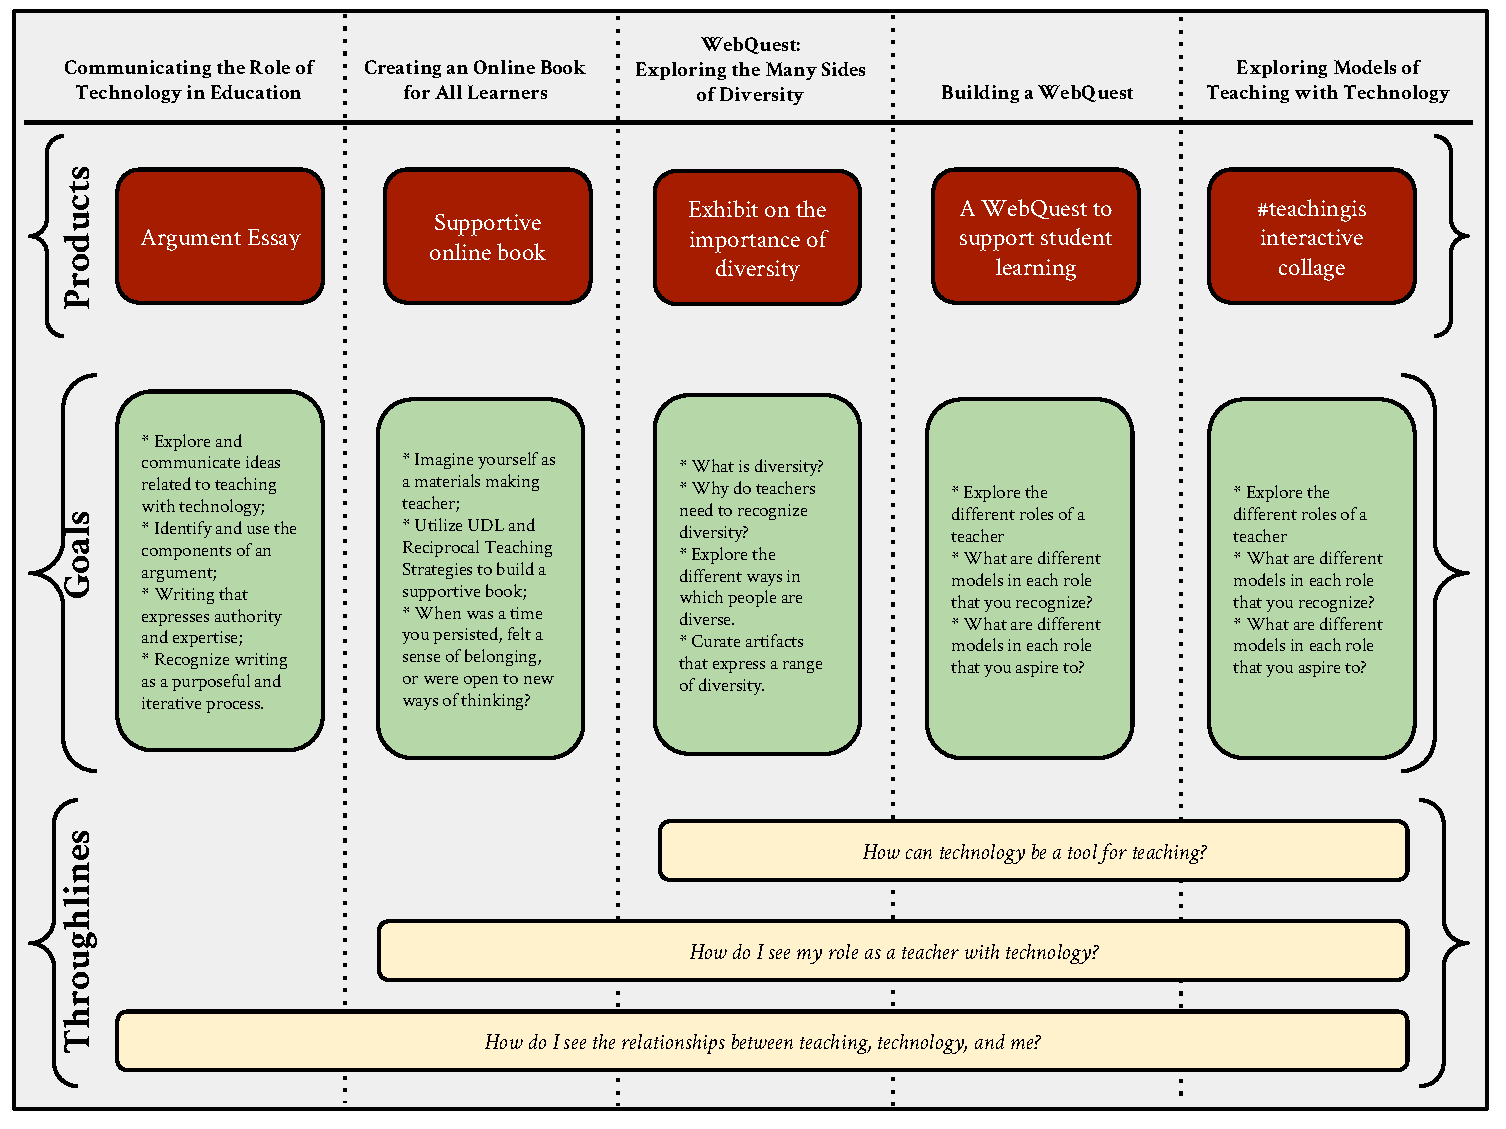
\includepdf[angle=90,width=6in]{course-map.pdf}

\newpage

\part{Appendix}

\begin{marginfigure}%
	\begin{center}
		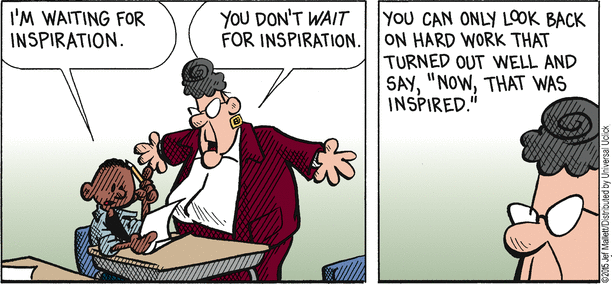
\includegraphics[width=1\linewidth]{frazz-inspiration.png}
	\end{center}
\end{marginfigure}

\section{Fairmont State School of Education Conceptual Framework}
The mission of the Fairmont State University School of Education (FSU SoE) is to prepare reflective and responsive educators who possess the knowledge, skills, and dispositions to help all students learn. The FSU SoE mission is integrated across the curriculum, field experiences, clinical practice, and assessments of candidates. The conceptual framework (CF) provides the structure and guiding principles that are necessary to accomplish this mission. The five West Virginia Professional Teaching Standards (WVPTS) and their respective functions undergird the knowledge, skills, and dispositions that candidates must possess in order to facilitate learning for all students. Diversity and technology are included in the CF representing themes that are integrated throughout the unit's programs. Demonstrated competencies in the standards/functions empower candidates to function as reflective and responsive educators. The CF is based on research about effective teaching and learning best practices that apply to teacher candidates at the initial level as well as accomplished teachers at the advanced level. The CF and the WVPTS also are central guiding elements of the FSU Professional Development School (PDS) Partnership that provides a critical structure and context for teacher education and educator professional development.

\begin{center}
\begin{figure}%
  \centerline{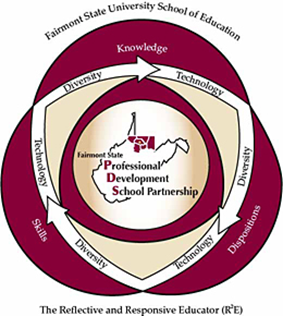
\includegraphics[width=0.5\linewidth]{fsu-cf.png}}
  \caption{Fairmont State University School of Education Conceptual Framework}
  \label{fig:fsu-cf}
\end{figure}
\end{center}

\section{Fairmont State University Policies}

\subsection{Academic Integrity}

Fairmont State values highly the integrity of its student scholars. All students and faculty members are urged to share in the responsibility for removing every situation which might permit or encourage academic dishonesty. Cheating in any form, including plagiarism, must be considered a matter of the gravest concern. Cheating is defined here as: the obtaining of information during an examination; the unauthorized use of books, notes, or other sources of information prior to or during an examination; the removal of faculty examination materials; the alteration of documents or records; or actions identifiable as occurring with the intent to defraud or use under false pretense. Plagiarism is defined here as: the submission of the ideas, words (written or oral), or artistic productions of another, falsely represented as one's original effort or without giving due credit. Students and faculty should examine proper citation forms to avoid inadvertent plagiarism.

\subsection{Disability Services}

Disability services are available to any student, full or part-time, who has a need because of a documented disability. It is the student's responsibility to register for disability services and to provide any necessary documentation to verify a disability or the need for accommodations. Students must provide their professors with a copy of their academic accommodation letter each semester in order to receive accommodations. Faculty, students, and the Office of Disability Services must cooperate to ensure the most effective provision of accommodations for each class.

The Office of Disability Services is located in suite 316 of the Turley Student Services Center 333-3661. For additional information, please visit the Fairmont State University Office of Disability Services webpage at www.fairmontstate.edu/access or call (304) 333-3661.

\end{document}